
\documentclass[sigconf,review]{acmart}
%
% defining the \BibTeX command - from Oren Patashnik's original BibTeX documentation.
%\def\BibTeX{{\rm B\kern-.05em{\sc i\kern-.025em b}\kern-.08emT\kern-.1667em\lower.7ex\hbox{E}\kern-.125emX}}
    
%\copyrightyear{2019}
%\acmYear{2019}
%\setcopyright{acmlicensed}
%\acmConference[SC '19]{SC '19: ACM Symposium on Neural Gaze Detection}{June 03--05, 2018}{Woodstock, NY}
%\acmBooktitle{Woodstock '18: ACM Symposium on Neural Gaze Detection, June 03--05, 2018, Woodstock, NY}
%\acmPrice{15.00}
%\acmDOI{10.1145/1122445.1122456}
%\acmISBN{978-1-4503-9999-9/18/06}



\usepackage{times}
\usepackage{t1enc}
\usepackage{todonotes}
\usepackage{graphicx}
\usepackage{epstopdf}
\usepackage{hyperref} % hyperlinks for references.
\usepackage{amssymb,amsmath,amsthm,amsfonts} % easier math formulae, align, subequations \ldots
\usepackage[vlined,ruled]{algorithm2e}

\usepackage{subcaption}
%\usepackage{algorithm}
\usepackage{algorithmic}

\begin{document}                     

\newif\ifcmts
\cmtstrue % comment out to hide answers

\newcommand{\tablefont}{\fontsize{6}{6}\selectfont}

%
% The "title" command has an optional parameter, allowing the author to define a "short title" to be used in page headers.
\title{Efficient Two Trees to Optimize Collectives: Broadcast, Reduce, and Allreduce}

%
% The "author" command and its associated commands are used to define the authors and their affiliations.
% Of note is the shared affiliation of the first two authors, and the "authornote" and "authornotemark" commands
% used to denote shared contribution to the research.
%\author{Ben Trovato}
%\authornote{Both authors contributed equally to this research.}
%\email{trovato@corporation.com}
%\orcid{1234-5678-9012}
%\author{G.K.M. Tobin}
%\authornotemark[1]
%\email{webmaster@marysville-ohio.com}
%\affiliation{%
%  \institution{Institute for Clarity in Documentation}
%  \streetaddress{P.O. Box 1212}
%  \city{Dublin}
%  \state{Ohio}
%  \postcode{43017-6221}
%}
%
%\author{Lars Th{\o}rv{\"a}ld}
%\affiliation{%
%  \institution{The Th{\o}rv{\"a}ld Group}
%  \streetaddress{1 Th{\o}rv{\"a}ld Circle}
%  \city{Hekla}
%  \country{Iceland}}
%\email{larst@affiliation.org}

%
% The abstract is a short summary of the work to be presented in the article.
\begin{abstract}
Text of abstract \ldots.
\end{abstract}


%
% The code below is generated by the tool at http://dl.acm.org/ccs.cfm.
% Please copy and paste the code instead of the example below.
%
%\begin{CCSXML}
%<ccs2012>
% <concept>
%  <concept_id>10010520.10010553.10010562</concept_id>
%  <concept_desc>Computer systems organization~Embedded systems</concept_desc>
%  <concept_significance>500</concept_significance>
% </concept>
% <concept>
%  <concept_id>10010520.10010575.10010755</concept_id>
%  <concept_desc>Computer systems organization~Redundancy</concept_desc>
%  <concept_significance>300</concept_significance>
% </concept>
% <concept>
%  <concept_id>10010520.10010553.10010554</concept_id>
%  <concept_desc>Computer systems organization~Robotics</concept_desc>
%  <concept_significance>100</concept_significance>
% </concept>
% <concept>
%  <concept_id>10003033.10003083.10003095</concept_id>
%  <concept_desc>Networks~Network reliability</concept_desc>
%  <concept_significance>100</concept_significance>
% </concept>
%</ccs2012>
%\end{CCSXML}
%
%\ccsdesc[500]{Computer systems organization~Embedded systems}
%\ccsdesc[300]{Computer systems organization~Redundancy}
%\ccsdesc{Computer systems organization~Robotics}
%\ccsdesc[100]{Networks~Network reliability}

%
% Keywords. The author(s) should pick words that accurately describe the work being
% presented. Separate the keywords with commas.
\keywords{MPI Collectives, two trees, broadcast, reduce, allreduce}

%
% A "teaser" image appears between the author and affiliation information and the body 
% of the document, and typically spans the page. 

%
% This command processes the author and affiliation and title information and builds
% the first part of the formatted document.
\maketitle

\section{Introduction}
%Efficient execution of processes and communication of data between them are two important goals of designing parallel applications for high performance computing system (HPC). Often, the performance of communication operations significantly affects the efficient execution of processes, and hence, the parallel application. 
Collective operations are among the most important communication operations for parallel applications running on large scale high performance computing systems. In general, all of the processes in a parallel application are involved in a collective operation either to send and/or receive data from other processes. A few widely used collective operations are: distributing identical data to all processes (i.e., broadcast), receiving different/identical data from all processes at the root process (i.e., gather/reduce) and also, to distribute the collected data (at the root) to all the processes (i.e., Allgather, Allreduce), etc.  Typically, acceleration of a parallel application involves optimizing collective operations.

Many virtual topologies have been used in the past for runtime optimization of collective operations \cite{hoefler-moor-collectives}. Among them, pipelined tree algorithms have been observed to reduce the runtime of various collectives which involves medium to large message sizes. The message to be sent (or received) is divided into small chunks and is distributed in a pipeline along the edges of the virtual topology.  Binary and linear trees are commonly used as virtual topologies for medium and large message sizes respectively. 

Sanders et. al. in \cite{sanders_two-tree_2009} observed that in a binary tree, the leaf nodes utilize only half of their bandwidth. When these nodes are receiving (in broadcast), they never send any message and while sending (in gather, reduce) no receive operation is performed. To fully utilize the bandwidth of these nodes, they proposed a two-tree based approach (referred as TwoTreeS in the paper). To perform a collective, instead of one, two binary trees are used. The inner nodes of one tree becomes the outer nodes in the other tree and hence, bandwidth of all the nodes can be fully utilized. 

The construction of TwoTreeS is rather complex and depends on perfect synchronization of send and receive operations in both the trees. The algorithm divides the communication in rounds. In each round, a process is receiving in one tree (referred as $T_1$) and sending to some other process in the second tree (referred as $T_2$). In a large communication network, perfect synchronization of send/receive operations in both the trees is not possible because of variable number of hops among processes and also due to traffic from other applications sharing the communication infrastructure. However, performing the communication in rounds to achieve synchronization becomes an overhead and does not allow to fully optimize the bandwidth with two trees. In this paper, we propose a simple construction of two trees which is named as Two Tree Complete (TwoTreeC) that does not depend on any direct or indirect synchronization of send/receive operations. We implement three widely used collectives: broadcast, reduce and allreduce using the proposed TwoTreeC algorithm. Major contributions of this work are as follows:

\begin{itemize}
\item A runtime efficient implementation of broadcast, reduce and allreduce collectives with an easy to implement two tree topology.
\item A close to lower bound and stable implementation of reduce and allreduce collectives for power of two and non power of two cases.
\item An exhaustive experimental evaluation of the proposed collectives on state-of-the-art high performance computing (HPC) system Piz Daint. \ifcmts \{\textcolor{blue}{todo}\} other HPC systems \fi
\item An empirical and simulator based calculation of number of chunks based on LogGP \cite{alexandrov_loggp:_1995} model.
\ifcmts \item \{\textcolor{blue}{todo}\} Speed-up of training deep learning models using the proposed allreduce implementation. \fi
\end{itemize}


%The Message Passing Interface (MPI) provides an implementation of commonly used collective operations.

%terminology: Sander's Two-Tree = TwoTreeS, Our Two-Tree = TwoTreeC.  Maybe T$_1$ and T$_2$ so that it is easy to refer to them throughout the rest of the paper?


%In Section \ref{sec:Model} we briefly explain the cost model LogGP \#ref\# that we have used in the analysis of our algorithms. Section \ref{sec:Topology} details the structure of our version of the two-tree topology adapted from Sanders and Traff's two-tree \#ref\#. Section \ref{sec:Operations} and its subsections illustrate how the two-tree is worked upon to carry out three basic collective operations: broadcast, reduce and all-reduce. Since this is a pipelined implementation, Section \ref{sec:Chunks} explains the process of calculation of the optimal number of chunks that we divide the message into for pipelining purpose. Section \ref{sec:Results} concludes with experimental results for all three operations.\\

%ToDo add: 1.explain all three operations.\\2.explain bandwidth drawback of binary tree.\\3.explain need for calculating optimal number of chunks in  pipeline.\\


\section{Motivation}\label{sec:Motivation}
The main idea behind two trees algorithm is to maximize the bandwidth utilization in a collective by using two binary trees referred as $T_1$ and $T_2$. The TwoTreeS algorithm constructs both $T_1$ and $T_2$ in such a way that the inorder traversal of $T_1$ is same in reverse of the inorder traversal of $T_2$. With this approach, the leafs of $T_1$ becomes the inner nodes of $T_2$ (refer Figure \ref{fig:twoTreeSandC}(a,b)). The message to be communicated is halved between the two trees and the halved message is sent by dividing it into smaller chunks to achieve efficiency. Hence, theoretically, doubling the bandwidth utilization than binary trees. To impose an indirect synchronization, the edges in both the trees are coloured to ensure that each node is receiving from some node in one tree and at the same time sending to some other node in the other tree. For each node, this send and receive operation together is called as a round and the entire communication is a collection of rounds. However, because of being a pipelined algorithm, sending of a chunk (part of the message) in a round depends on receiving the same chunk in the previous round. Following we highlight some major drawbacks of the TwoTreeS approach.

\begin{figure*}[t]
 
\begin{tabular}{cccc}
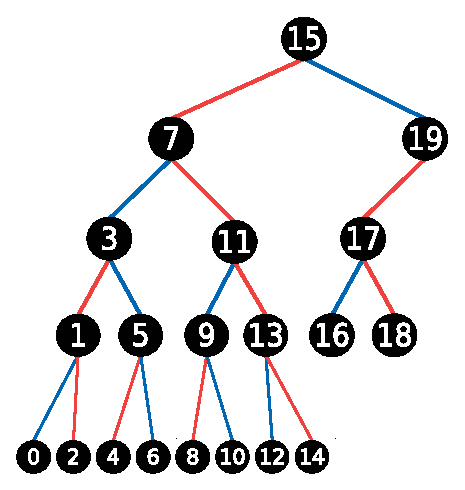
\includegraphics[scale=0.47]{images/unbalanced-S-T1-gap.eps}  & \hspace{0.4cm} 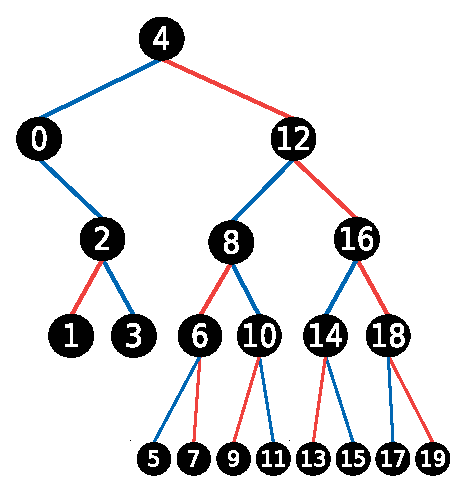
\includegraphics[scale=0.47]{images/unbalanced-S-T2-gap.eps} & 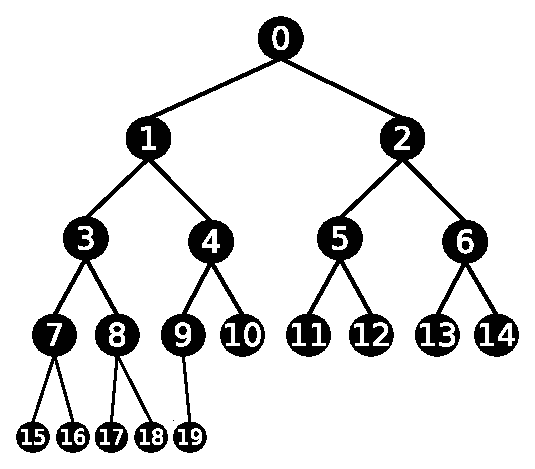
\includegraphics[scale=0.49]{images/complete-T1-gap.eps} &  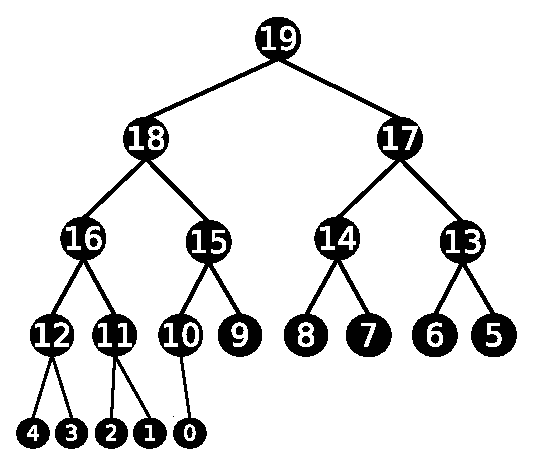
\includegraphics[scale=0.49]{images/complete-T2-gap.eps} \\ \\
(a) $T_1$ in TwoTreeS & (b) $T_2$ in TwoTreeS & (c) $T_1$ in TwoTreeC & (d) $T_2$ in TwoTreeC \\ \\
\end{tabular}
\caption{Design of two trees $T_1$ and $T_2$ for $20$ processes in (a,b) TwoTreeS \cite{sanders_two-tree_2009} and (c,d) TwoTreeC}
\label{fig:twoTreeSandC}
\end{figure*}

\begin{description}
    \item[$\bullet$]TwoTreeS suffers from an overhead of indirect synchronization due to the colouring of edges. Colouring ensures that the communication goes round by round in a synchronized way. However, synchronization might add delays due to underlying network traffic. We have implemented TwoTreeS both with colouring based schedule (TwoTreeS\_Bottom and TwoTreeS\_Top) and completely unsynchronized using our approach (TwoTreeS\_Unsync), results clearly state that the overhead of synchronization is more than its benefit.
%    \item[$\bullet$]TwoTreeS does not ensure proper balancing of tree, which could result in reduced bandwidth utilization in cases with non power of two number of processes. Effects were evident especially in reduce and allreduce when one sub-tree becomes significantly shorter than the other. Figure \ref{fig:twoTreeS} illustrates this imbalance for $21$ processes.
    \item[$\bullet$]As described in the article \cite{sanders_two-tree_2009}, in a particular case of total \(2^n+1\) processes for a rooted collective operation, the two trees are constructed such that there is a complete binary tree of \(2^n-1\) processes, and one extra node at the top. Thus, this extra node has only one child on the left in $T_1$ and the right in $T_2$. Later, root process node is also put on the top.  Hence, extra latency is added to the pipeline. We refer to this version of TwoTreeS as TwoTreeS\_Top and to understand the impact of this latency, we added this extra node at the bottom of the complete tree for this specific case only. This variation is named as  TwoTreeS\_Bottom.
    \item[$\bullet$]The topology construction time for TwoTreeS is relatively higher, especially, the colouring algorithm.
\end{description}

The potential of two trees mechanism in general and issues concerning TwoTreeS implementation has motivated the development of the proposed algorithm, TwoTreeC. We discuss the construction of two trees with TwoTreeC in the next section.

\section{Two Tree Complete (TwoTreeC)}\label{sec:TwoTreeC}
The idea behind TwoTreeC is rather very simple. We construct two complete binary trees $T_1$ and $T_2$ each using $P$ processes. In a rooted collective, these two trees are then assigned as left and right sub-tree of the root process. $T_1$ and $T_2$ are constructed as follows:
\begin{description}
    \item[$\bullet$]The trees are designed in such a way that leaf nodes in one tree are the inner nodes in the other and vice-versa.
    \item[$\bullet$]$T_1$(left tree) is numbered level wise, left to right, with increasing process id's starting from $0$.
    \item[$\bullet$]$T_2$(right tree) is numbered level wise, left to right, with decreasing process id's starting from $P-1$.
\end{description}
Here $P$ is the total number of processes. An example $T_1$ and $T_2$ for $20$ processes using TwoTreeC is shown in figure \ref{fig:twoTreeSandC} (c,d). Each process independently uses Algorithm \ref{alg:TwoTreeComp} to compute its parent and children in $T_1$ and $T_2$. With the exception of the root process, the remaining processes appear in both left and right trees. Therefore, $leftParent$ is used to denote parent of current process in left tree, and $rightParent$ is the parent of current process in right tree. $leftChild[]$ and $rightChild[]$ similarly denote the children of current node in left and right tree respectively. 

\begin{algorithm}
\algsetup{linenosize=\tiny}
 \scriptsize
\caption{Two Tree Complete Construction}\label{alg:TwoTreeComp}
\begin{algorithmic}[1]
\REQUIRE Number of processes $\leftarrow$ \(p\), rank $\leftarrow processId$ 
\IF{$rank$ = 0}
    \STATE numberOfLeftChildren $ \leftarrow 1$
    \STATE numberOfRightChildren $ \leftarrow 1$
    \STATE leftChild$[0] \leftarrow 1$
    \STATE rightChild$[0] \leftarrow p-1$
\ELSE[$rank \neq 0$]
    \STATE leftParent $ \leftarrow rank / 2$
    \STATE rightParent $ \leftarrow \big(p-\dfrac{p-rank}{2}\big)\%p$
    \IF{$(2 \times rank) < p$}
         \STATE numberOfLeftChildren $ \leftarrow 1$
         \STATE leftChild[0]$ \leftarrow 2 \times rank$
    \ENDIF
    \IF{$\big((2 \times rank) + 1\big) < p$}
         \STATE numberOfLeftChildren $ \leftarrow 2$
         \STATE leftChild[1]$ \leftarrow \big((2 \times rank) + 1\big)$
    \ENDIF
    \IF{$\big((2 \times rank) - p\big) > 0$}
         \STATE numberOfRightChildren $ \leftarrow 1$
         \STATE rightChild$[0] \leftarrow \big((2 \times rank) - p\big)$
    \ENDIF
    \IF{$\big((2 \times rank) - p - 1\big) > 0$}
         \STATE numberOfRightChildren $ \leftarrow 2$
         \STATE rightChild$[1] \leftarrow \big((2 \times rank) - p - 1\big)$
    \ENDIF
\ENDIF
\end{algorithmic}
\end{algorithm}

TwoTreeC implementation addresses all the observed issues with TwoTreeS. There is no overhead due to colouring or synchronization, because we perform no explicit/implicit synchronization. The construction of trees takes only O(1) time on each process.
%Throughout all of the implementation, all the send and receive operations used are non-blocking.
%Both the trees are relatively balanced than TwoTreeS. The impact of balancing has been seen in performance gain of reduce and allreduce collectives since, the communication begins at the leaf nodes in both of the collectives.

\section{Collectives with TwoTreeC}\label{sec:Operations}
The TwoTreeC topology discussed above is used to implement broadcast, reduce and allreduce operations. The broadcast and reduce operations are rooted collectives i.e., the data is either distributed by the root process (ex., broadcast) or is collected at the root process (as in reduce). We implement allreduce as a combination of broadcast and reduce collectives. Similar to binary pipeline algorithm, TwoTreeC divides message into smaller chunks and communicate the chunks in a pipeline. We describe the approaches used to calculate number of chunks for various collectives in section \ref{sec:Chunks}.  Figure \ref{fig:towtreeC_coll} depicts our basic approach to perform these collectives using TwoTreeC. Assuming the entire message is divided into $m$ small chunks, in broadcast, even numbered chunks are sent to tree $T_1$ one after the other in a pipeline. Similarly, odd numbered chunks are sent to sub-tree $T_2$. The chunks travel from leaf processes to the root in the reduce collective. Whereas, in allreduce, reduce of the entire message happens at the root process which is followed by the pipelined broadcast. More details about each of the collectives is presented below.

%\ifcmts \{\textcolor{blue}{todo @Mohit LogGP analysis for each of these approaches.}\}

\begin{figure}[h]
 
\begin{tabular}{cc}
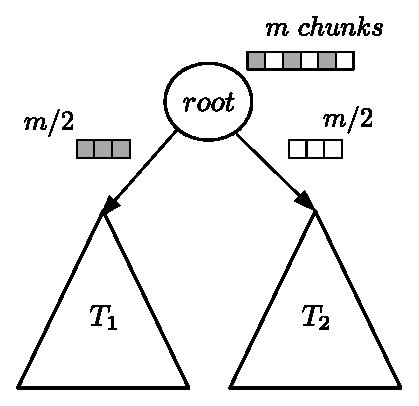
\includegraphics[scale=0.46]{images/ttbroad.eps} &  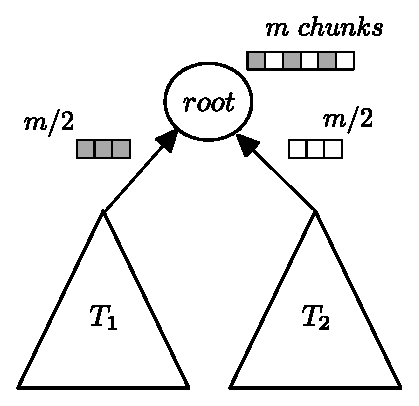
\includegraphics[scale=0.46]{images/ttreduce.eps} \\ \\
(a) Broadcast & (b) Reduce \\
\end{tabular}
\caption{Broadcast and reduce with TwoTreeC}
\label{fig:towtreeC_coll}
\end{figure}

\subsection{Broadcast} \label{sec:broad}
In broadcast collective, a message from the root process is received at all other processes in the communicator. In case rank $0$ is the root process of the collective then each process execute algorithm \ref{alg:TwoTreeComp} to find its parent and children in tree $T_1$ and $T_2$. All other processes other than the root process are available in both $T_1$ and $T_2$. Later, processes perform send and receive operations using algorithm \ref{alg:broadcastImpl}. In case the root of a rooted collective is not the process ranked $0$ but some other process $k$, then each process assumes a false rank $(rank-k)\%P$ and finds the false ranks of its parents and children using algorithm \ref{alg:TwoTreeComp}. These false ranks are translated back to original ranks using the same modulo function. 

The root node divides its data into a number of equal sized chunks, then one by one sends each odd-numbered chunk to the root of $T_2$ (right subtree) and each even-numbered chunk to the root of $T_1$ (left subtree). Non-root processes expect odd numbered chunks from $leftParent$ and upon receiving, forward them to their $leftChild[0]$ and $leftChild[1]$. Same task is performed in the right subtree. In the end, each process has received all the chunks, odd ones in the right tree and even ones in the left subtree.

\begin{algorithm}
\algsetup{linenosize=\tiny}
  \scriptsize
\caption{Two Tree Broadcast operation}\label{alg:broadcastImpl}
\begin{algorithmic}[1]
\REQUIRE rank $\leftarrow processId$ 
\IF{$rank$ = root}
    \FORALL{Chunks}
        \IF{Even Chunk} 
            \STATE Non-blocking send this chunk to leftChild[0]
        \ELSE
            \STATE Non-blocking send this chunk to rightChild[0]
        \ENDIF
    \ENDFOR
\ELSE[$rank \neq root$]
    \FORALL{Chunks}
        \IF{Even Chunk} 
            \STATE Non-blocking receive this chunk from leftParent
        \ELSE[Odd Chunk]
            \STATE Non-blocking receive this chunk from rightParent
        \ENDIF
    \ENDFOR
    \WHILE{all chunks not received}
        \STATE Wait until any of the receives finishes
        \IF{Even chunk received}
            \STATE Non-blocking send this chunk to leftChild[0] and leftChild[1]
        \ELSE[Odd chunk received]
            \STATE Non-blocking send this chunk to rightChild[0] and rightChild[1]
        \ENDIF
    \ENDWHILE
\ENDIF
\STATE Wait on all sends to finish
\end{algorithmic}
\end{algorithm}

\subsection{Reduce}
We use TwoTreeC to implement commutative and associative reduce collective. In reduce collective as well, we use the similar process as described in section \ref{sec:broad} for broadcast to design two trees $T_1$ and $T_2$. Similarly, $T_1$ is placed as the left subtree of the root of the collective and  $T_2$ as the right subtree. The leaf nodes begins the reduce operation by sending chunks of messages to the parent nodes as depicted in figure \ref{fig:towtreeC_coll}(b). Each non-leaf node receives the chunk number say $m$ from the child nodes and then perform the reduce operation together with its own $m^{th}$ chunk. The reduced chunk is then forwarded to the parent node and eventually reaches the root of the tree. 

\subsection{Allreduce}
We have implemented allreduce operation by doing reduce of all the chunks at the root node and then doing a broadcast. We assume process with rank $0$ to be our root process. The trees $T_1$ and $T_2$ are designed as already explained in section \ref{sec:broad}. Both of these trees are used to perform pipelined reduce operation. As soon as the root process receives any of the reduced chunk, it performs the broadcast using the same $T_1$ and $T_2$ (refer Figure \ref{fig:towtreeC_allreduce}). By doing this overlap of reduce and broadcast operations, we further improve time efficiency of our implementation as compared to first wait for all the chunks to be reduced at the root process and then beginning to broadcast. 

\begin{figure}[t]
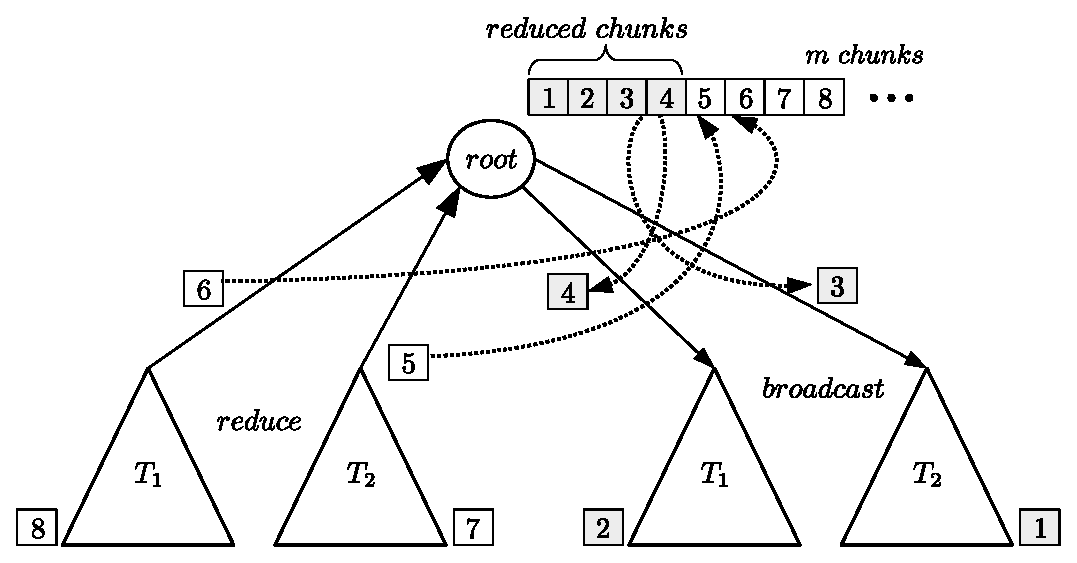
\includegraphics[scale=0.46]{images/ttallreduce.eps} \\ 
\caption{Allreduce with TwoTreeC showing overlap of reduce and broadcast}
\label{fig:towtreeC_allreduce}
\end{figure}

As can be seen in figure \ref{fig:towtreeC_allreduce}, to implement allreduce collective, two pairs of two-trees have been used. Instead of using the same pair of $T_1$ and $T_2$ for both reduce and broadcast, different pairs can also be used to further improve the time efficiency. We have designed and tested two variations of our original TwoTreeC allreduce implementation which uses different pairs for reduce and broadcast phases. 


\subsubsection{TwoTreeC+C}
The main idea behind TwoTreeC+C allreduce implementation is to improve the bandwidth utilization of the leaf nodes in the reduce phase of TwoTreeC. We design a new pair of two trees for broadcast phase (referred as $T_3$ and $T_4$) such that the nodes finishing the reduce part first in $T_1$ are closer to the root node in $T_3$ and $T_4$. The two trees for reduce phase in TwoTreeC+C is same as that of $T_1$ and $T_2$ in TwoTreeC. We have designed $T_3$ and $T_4$ (complete trees) for broadcast phase of TwoTreeC+C as follows:

\begin{description}
     \item[$\bullet$]T$_{3}$ is numbered in level wise, in increasing order (circular in range $1...P-1$) starting from $\left \lceil{\dfrac{P}{2}}\right \rceil$
     \item[$\bullet$] T$_{4}$ is numbered in level wise, in decreasing order (circular in range $1...P-1$) starting from $\left \lfloor{\dfrac{P}{2}}\right\rfloor $
 \end{description}
Figure \ref{fig:reordered} shows $T_3$ and $T_4$ for TwoTreeC+C for 20 processes.

\begin{figure}[t]
\begin{tabular}{cc}
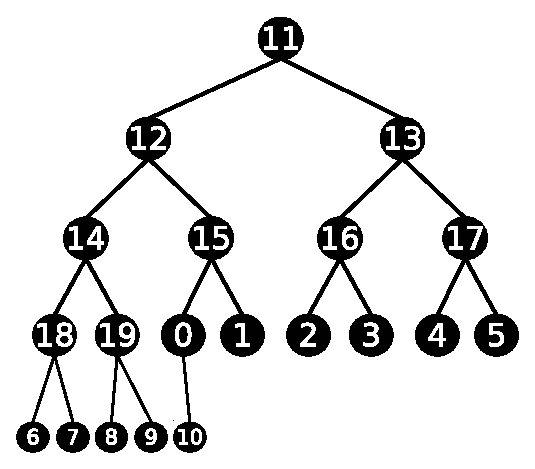
\includegraphics[scale=0.46]{images/reordered-twoTreeC-T1.eps} &  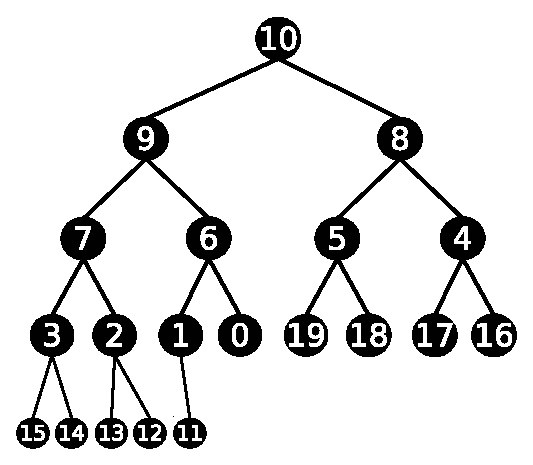
\includegraphics[scale=0.46]{images/reordered-twoTreeC-T2.eps} \\ \\
(a) $T_3$ & (b) $T_4$ \\
\end{tabular}
\caption{$T_3$ and $T_4$ for TwoTreeC+C for 20 processes}
\label{fig:reordered}
\end{figure}

\subsubsection{TwoTreeC+S}
Both TwoTreeC and TwoTreeS uses totally different methods to achieve the same objective of designing pair of two trees. This version of allreduce is a random choice of using both of the topologies together. The $T_1$ and $T_2$ trees uses TwoTreeC topology whereas $T_3$ and $T_4$ are designed using TwoTreeS topology. The basic idea is to get benefit from both of the topologies. However, instead of using coloring for synchronization in TwoTreeS, we only make use of TwoTreeS topology exactly similar to TwoTreeC i.e., in an unsynchronized way as described in algorithm \ref{alg:broadcastImpl}. 

\section{Calculating Number of Chunks} \label{sec:Chunks}
An important component of any pipelined collective is to optimally divide the message in to smaller number of chunks. The number of chunks and hence, the size of each chunk are important factors affecting runtime. %Calculating the chunks value for different algorithms and for different parameters was also very challenging. 
We have tried and tested following three approaches to calculate the best possible chunk value for the proposed algorithm for varying message size and number of processes. All of these approaches are based on modelling the runtime of the algorithm based on LogGP \cite{alexandrov_loggp:_1995} parameters viz: L:Latency; o:cpu overhead; g: gap between messages; G: gap per byte; P: number of processes. To evaluate these parameters for an HPC system, netgauge tool \cite{hoefler_w.:_2007} is used. The values of these parameters along with optimal chunk values for each algorithm is described in the results section.

%Testing 1025 bytes 100 times:
%L = 1.589921 s = 1025 o_s = 1.709757 o_r = 1.711930 g = 1.346026 G = 0.000362 (21.564100 GiB/s) lsqu(g,G) = -nan
%  6:23 PM
%
%This was the original result calculated from daint
%  6:25 PM
%
%For simulator we used the values given by salvo
%L=1623300
%O=100
%G=100

\subsection{Mathematical Approach}
The traditional approach to calculate optimal chunks for any pipelined collectives is to model the runtime of the collective using some known model of communication \cite{thakur_optimization_2005}. LogGP is an widely accepted model for communication. For example, the runtime ($T_{2T}$) of broadcast collective using TwoTreeC in LogGP parameters can be evaluated as follows: 
\begin{equation}
T_{2T} = L+3o+sG +  \log{}_2 P (L + 3o + \frac{sG}{2N}) + \mathcal{O}(N + s/2)
\end{equation}

where, $N$ is the number of chunks into which the message size $s$ is divided. This approach is mostly useful for theoretical comparison of algorithms. However, LogGP model does not include network traffic and other realistic parameters and is simply an approximation. Also, it is very difficult to accurately measure the LogGP parameters as discussed in \cite{hoefler_w.:_2007}. Hence, it is very less probable to get a near optimal value from this approach. 


\subsection{Simulation}
Another interesting choice is to simulate the send and receive operations in a collective using a simulator. LogGOPSim \cite{hoefler-loggopsim} simulator is based on LogGP model and has been widely used for simulating MPI collectives. 

\ifcmts \{\textcolor{red}{todo @Salvo To write more about LogGOPSim}\} \fi

\subsection{Random}
LogGOPSim simulator also does not model real network traffic and hence, is not always accurate to predict the optimal number of chunks as depicted experimentally. To have a more robust approach, we performed experiments using ($\pm$10\%, $\pm$20\%) of the optimal chunk value obtained from LogGOPSim. This approach helped us to cover a relatively larger range of chunk values and then choose the chunk value for which the collective finishes the fastest for different number of processes and message sizes. 

\section{Experiments and Results} \label{sec:results}
\ifcmts \{\textcolor{blue}{todo: LogGP parameter values, algorithm compared with, other details like single process per node, etc.}\}
%Mention and briefly explain all the implementations compared: linear pipeline, pipelined binary tree, our pipelined two tree, mpi standard library, scatter-gather. Conclude how our approach outperformes the rest on larger data sizes.

\subsection{Broadcast}


\begin{figure*}
\centering
\begin{subfigure}{.33\textwidth}
  \centering
  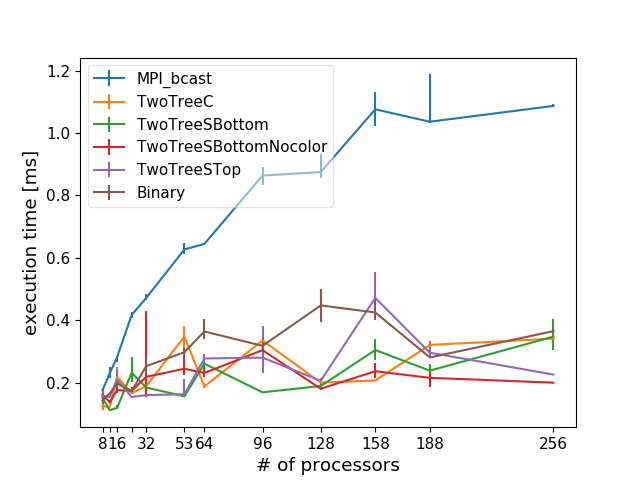
\includegraphics[width=1\linewidth]{images/Results/bcastFinal_262144B.png}
  \caption{Broadcast-256KB}
  \label{bcast-selected-256B}
\end{subfigure}%
\begin{subfigure}{.33\textwidth}% Text of paper \ldots
  \centering
  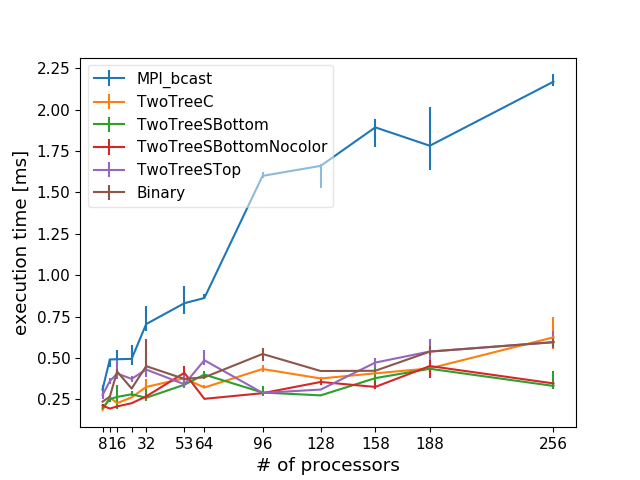
\includegraphics[width=1\linewidth]{images/Results/bcastFinal_524288B.png}
  \caption{Broadcast-512KB}
  \label{bcast-selected-512B}
\end{subfigure}
\begin{subfigure}{.33\textwidth}
  \centering
  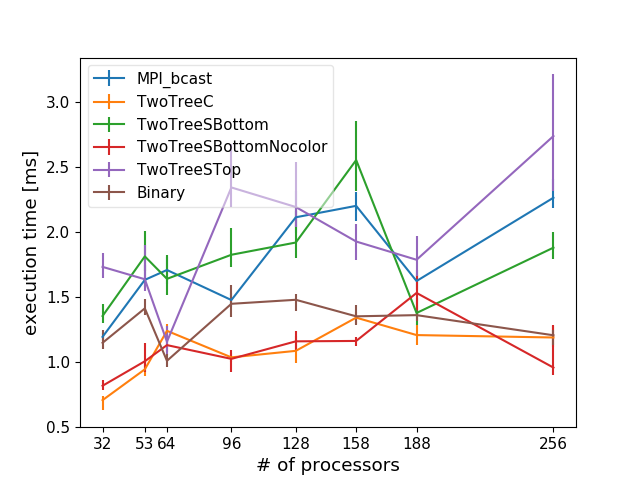
\includegraphics[width=1\linewidth]{images/Results/bcastFinal_1048576B.png}
  \caption{Broadcast-1MB}
  \label{bcast-selected-3MB}
\end{subfigure}%
\caption{Broadcast collective using small message sizes}
\label{graph-bcast-small-selected}
\end{figure*}

\begin{figure*}
\centering
\begin{subfigure}{.33\textwidth}
  \centering
  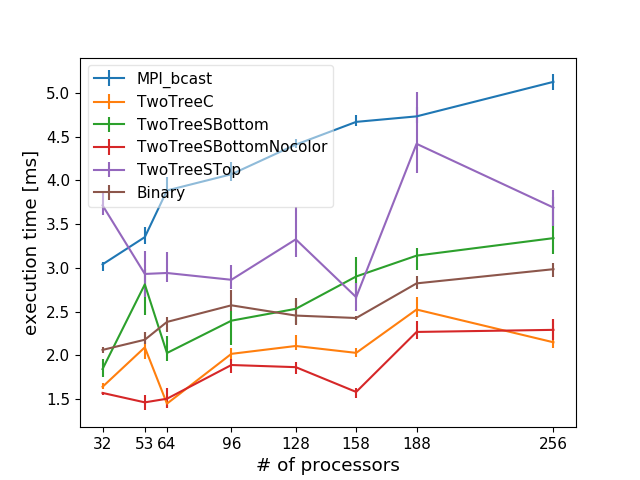
\includegraphics[width=1\linewidth]{images/Results/bcastFinal_3145728B.png}
  \caption{Broadcast-3MB}
  \label{bcast-selected-3MB}
\end{subfigure}
\begin{subfigure}{.33\textwidth}
  \centering
  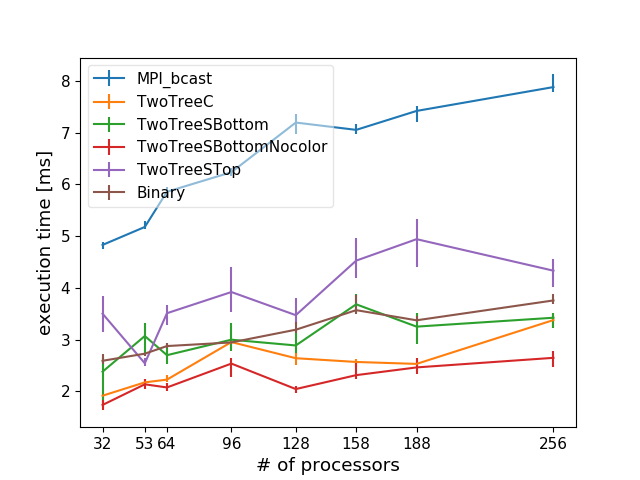
\includegraphics[width=1\linewidth]{images/Results/bcastFinal_5242880B.png}
  \caption{Broadcast-5MB}
  \label{bcast-selected-5MB}
\end{subfigure}%
\begin{subfigure}{.33\textwidth}
  \centering
  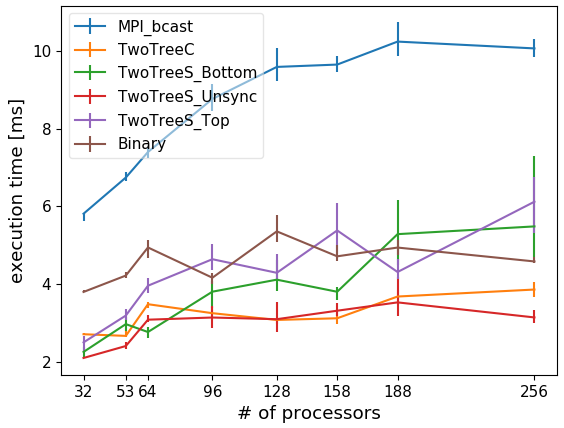
\includegraphics[width=1\linewidth]{images/Results/bcastFinal_7340032B.png}
  \caption{Broadcast-7MB}
  \label{bcast-selected-7MB}
\end{subfigure}
\caption{Broadcast collective using medium message sizes}
\label{graph-bcast-medium2-selected}
\end{figure*}



\subsection{Reduce}

\begin{figure*}
\centering
\begin{subfigure}{.33\textwidth}
  \centering
  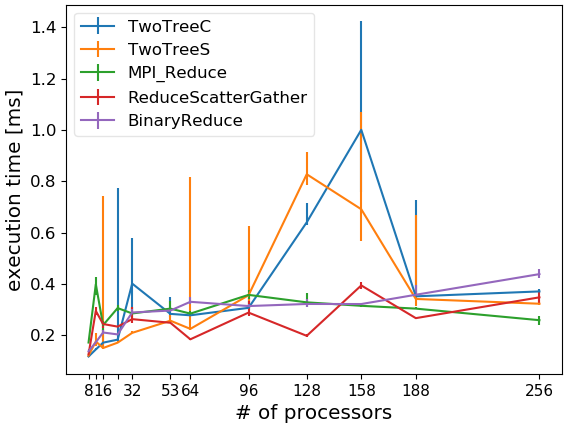
\includegraphics[width=1\linewidth]{images/Results/reducefinal_262144B.png}
  \caption{Reduce - 256KB}
  \label{reduce-selected-256B}
\end{subfigure}%
\begin{subfigure}{.33\textwidth}
  \centering
  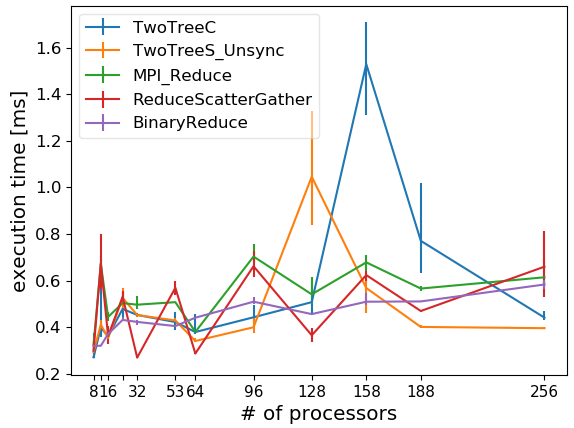
\includegraphics[width=1\linewidth]{images/Results/reducefinal_524288B.png}
  \caption{Reduce - 512KB}
  \label{reduce-selected-512B}
\end{subfigure}
\begin{subfigure}{.33\textwidth}
  \centering
  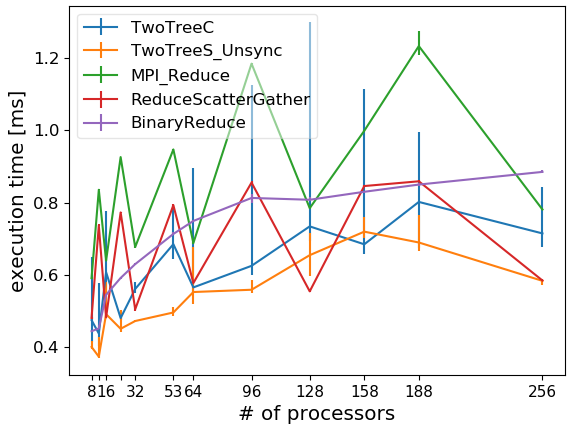
\includegraphics[width=1\linewidth]{images/Results/reducefinal_1048576B.png}
  \caption{Reduce - 1MB}
  \label{reduce-selected-1MB}
\end{subfigure}%
\caption{Reduce collective using small message sizes}
\label{graph-reduce-small-selected}
\end{figure*}

\begin{figure*}
\centering
\begin{subfigure}{.33\textwidth}
  \centering
  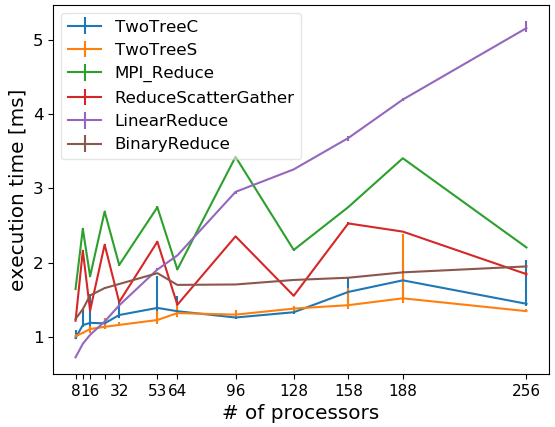
\includegraphics[width=1\linewidth]{images/Results/reducefinallinear_3145728B.png}
  \caption{Reduce - 3MB}
  \label{reduce-selected-3MB}
\end{subfigure}
\begin{subfigure}{.33\textwidth}
  \centering
  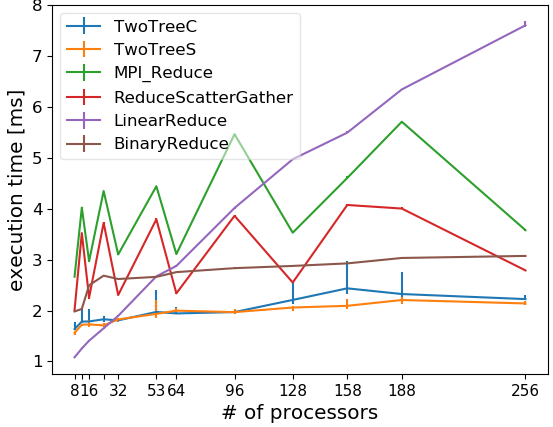
\includegraphics[width=1\linewidth]{images/Results/reducefinallinear_5242880B.png}
  \caption{Reduce - 5MB}
  \label{reduce-selected-5MB}
\end{subfigure}%
\begin{subfigure}{.33\textwidth}
  \centering
  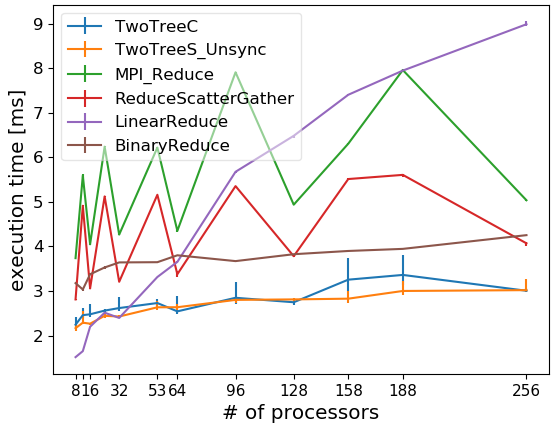
\includegraphics[width=1\linewidth]{images/Results/reducefinallinear_7340032B.png}
  \caption{Reduce - 7MB}
  \label{reduce-selected-7MB}
\end{subfigure}
\caption{Reduce collective using medium message sizes}
\label{graph-reduce-medium1-selected}
\end{figure*}


\subsection{All-Reduce}

\ifcmts \{\textcolor{red}{todo lower bound plot}\} \fi

\begin{figure*}
\centering
\begin{subfigure}{.33\textwidth}
  \centering
  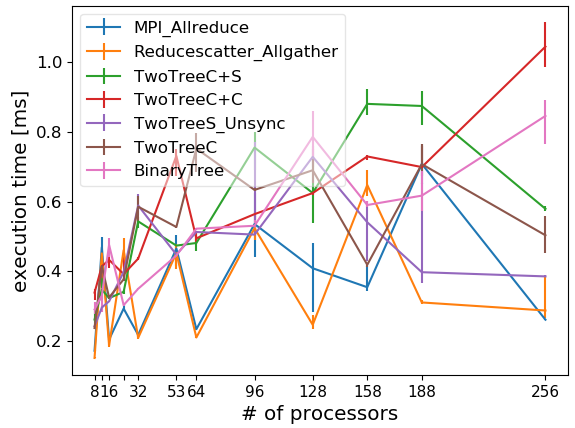
\includegraphics[width=1\linewidth]{images/Results/AllReduce/allreducecomp3_262144B.png}
  \caption{All-Reduce - 256KB}
  \label{reduce-selected-256B}
\end{subfigure}%
\begin{subfigure}{.33\textwidth}
  \centering
  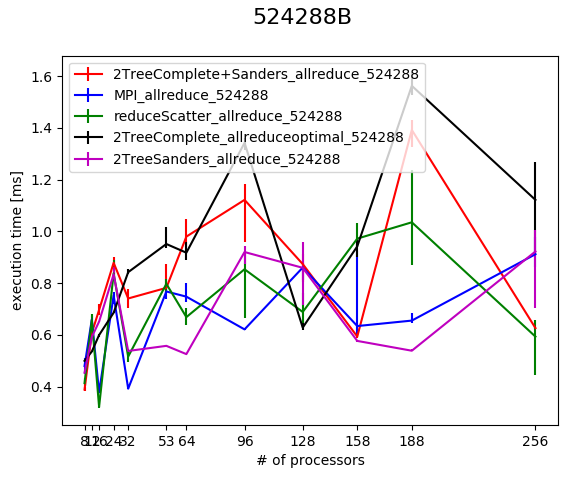
\includegraphics[width=1\linewidth]{images/Results/AllReduce/allreducecomp3_524288B.png}
  \caption{All-Reduce - 512KB}
  \label{reduce-selected-512B}
\end{subfigure}
\begin{subfigure}{.33\textwidth}
  \centering
  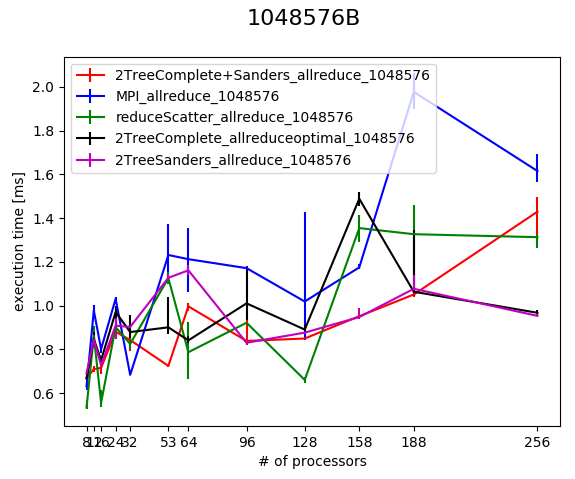
\includegraphics[width=1\linewidth]{images/Results/AllReduce/Allreduce_comp2_1048576B.png}
  \caption{All-Reduce - 1MB}
  \label{reduce-selected-1MB}
\end{subfigure}%
\caption{Allreduce collective using small message sizes}
\label{graph-reduce-small-selected}
\end{figure*}

\begin{figure*}
\centering
\begin{subfigure}{.33\textwidth}
  \centering
  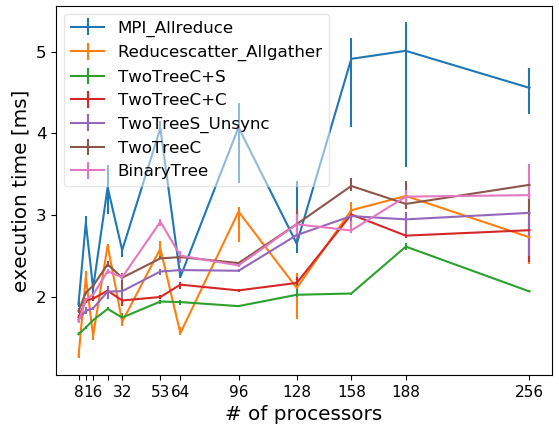
\includegraphics[width=1\linewidth]{images/Results/AllReduce/Allreduce_comp2_3145728B.png}
  \caption{All-Reduce - 3MB}
  \label{reduce-selected-3MB}
\end{subfigure}
\begin{subfigure}{.33\textwidth}
  \centering
  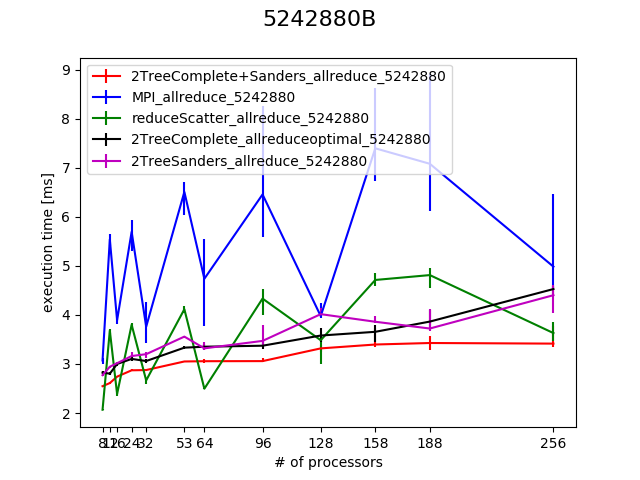
\includegraphics[width=1\linewidth]{images/Results/AllReduce/Allreduce_comp2_5242880B.png}
  \caption{All-Reduce - 5MB}
  \label{reduce-selected-5MB}
\end{subfigure}%
\begin{subfigure}{.33\textwidth}
  \centering
  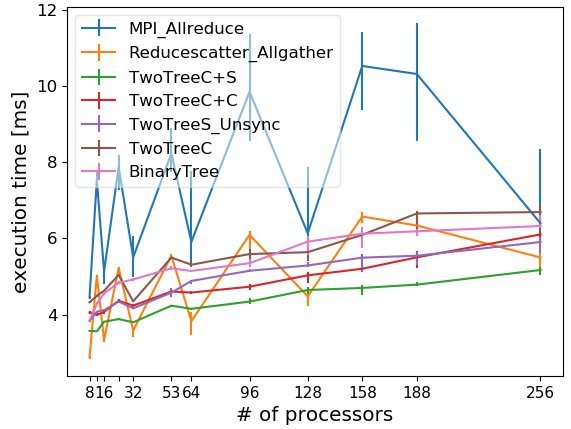
\includegraphics[width=1\linewidth]{images/Results/AllReduce/Allreduce_comp2_7340032B.png}
  \caption{All-Reduce - 7MB}
  \label{reduce-selected-7MB}
\end{subfigure}
\caption{Allreduce collective using medium message sizes}
\label{graph-reduce-medium1-selected}
\end{figure*}

\begin{figure*}
\centering
\begin{subfigure}{.33\textwidth}
  \centering
  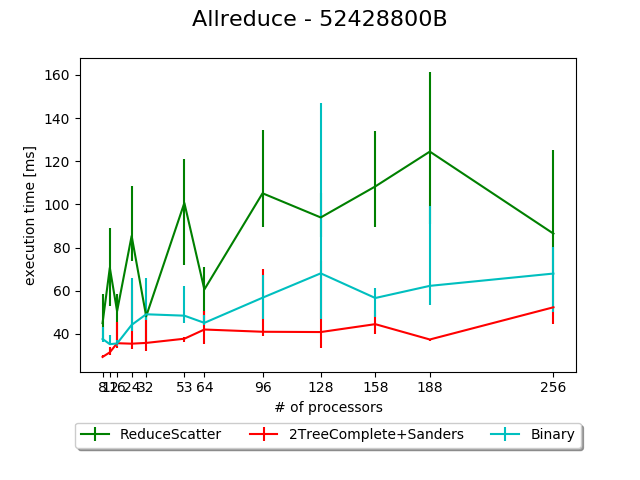
\includegraphics[width=1\linewidth]{images/Results/AllReduce/AllReduceComp2_52428800B.png}
  \caption{All-Reduce - 50MB}
  \label{reduce-selected-5MB}
\end{subfigure}%
\begin{subfigure}{.33\textwidth}
  \centering
  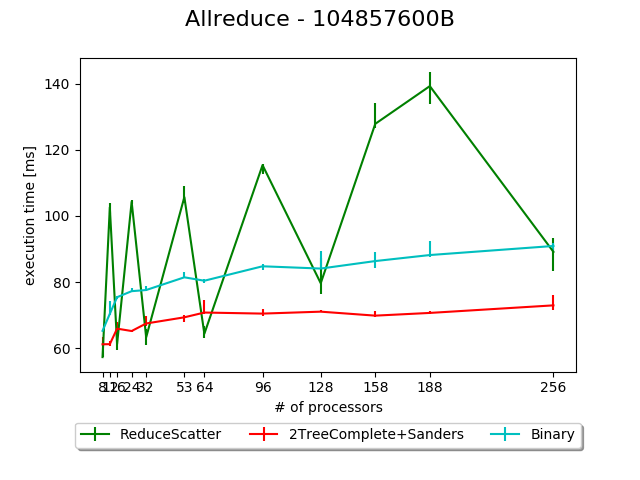
\includegraphics[width=1\linewidth]{images/Results/AllReduce/AllReduceComp2_104857600B.png}
  \caption{All-Reduce - 100MB}
  \label{reduce-selected-7MB}
\end{subfigure}
\begin{subfigure}{0.33\textwidth}
  \centering
  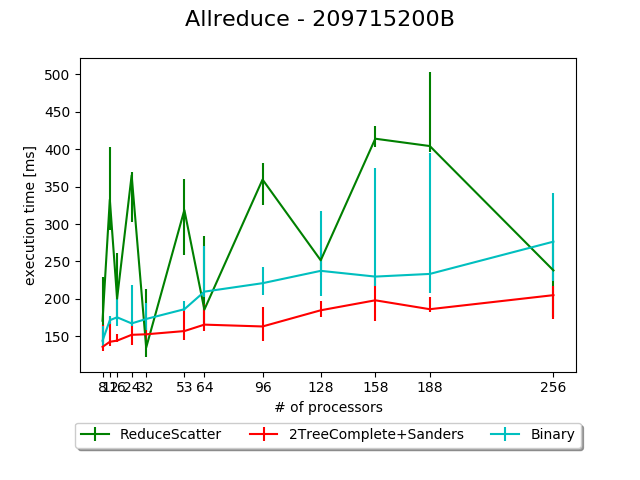
\includegraphics[width=1\linewidth]{images/Results/AllReduce/AllReduceComp2_209715200B.png}
  \caption{All-Reduce - 200MB}
  \label{reduce-selected-7MB}
\end{subfigure}
\caption{Allreduce collective using large message sizes}
\label{graph-reduce-medium2-selected}
\end{figure*}

\begin{table}[t]
\caption{No. of chunks used for TwoTreeC in Broadcast}
\begin{center}
\tablefont
\begin{tabular}{|c|c|c|c|c|c|c|c|c|c|}
\hline
& \multicolumn{8}{c|}{Number of Processes} \\
\hline
Size & 32 & 53 & 64 & 96 & 128 & 158 & 188 & 256\\
\hline
 256 KB & 4 & 7 & 10 & 14 & 6 & 6 & 10 & 10\\
 512 KB & 10 & 10 & 10 & 15 & 14 & 8 & 15 & 14\\
 1 MB & 8 & 8 & 16 & 16 & 15 & 15 & 15 & 12\\
 3 MB & 27 & 27 & 24 & 27 & 27 & 16 & 25 & 24\\
 5 MB & 20 & 45 & 45 & 45 & 45 & 45 & 45 & 45\\
 7 MB & 29 & 24 & 46 & 58 & 32 & 32 & 32 & 57\\
\hline
\end{tabular}
\end{center}
\end{table}

\begin{table}[]
\caption{No. of chunks used for TwoTreeC in Reduce}
\begin{center}
\tablefont
\begin{tabular}{|c|c|c|c|c|c|c|c|c|c|c|c|c|c|}
\hline
& \multicolumn{12}{c|}{Number of Processes} \\
\hline
Size & 8 & 12 & 16 & 24 & 32 & 53 & 64 & 96 & 128 & 158 & 188 & 256\\
\hline
 256 KB & 4 & 4 & 4 & 4 & 3 & 2 & 3 & 3 & 1 & 2 & 3 & 3\\
 512 KB & 4 & 4 & 4 & 4 & 4 & 6 & 12 & 9 & 9 & 12 & 12 & 12\\
 1 MB & 4 & 12 & 4 & 12 & 6 & 9 & 12 & 12 & 8 & 12 & 12 & 17\\
 3 MB & 14 & 10 & 18 & 22 & 15 & 24 & 15 & 30 & 40 & 24 & 24 & 30\\
 5 MB & 18 & 15 & 18 & 26 & 38 & 24 & 30 & 40 & 40 & 36 & 30 & 30\\
 7 MB & 14 & 20 & 34 & 26 & 38 & 24 & 40 & 30 & 40 & 30 & 52 & 40\\
\hline
\end{tabular}
\end{center}
\end{table}

\begin{table}[]
\caption{No. of chunks used for TwoTreeC+S in Allreduce}
\begin{center}
\tablefont
\begin{tabular}{|c|c|c|c|c|c|c|c|c|c|c|c|c|}
\hline
 & \multicolumn{12}{c|}{Number of Processes} \\
\hline
 Size & 8 & 12 & 16 & 24 & 32 & 53 & 64 & 96 & 128 & 158 & 188 & 256\\
\hline
 256 KB & 2 & 2 & 2 & 2 & 2 & 2 & 2 & 2 & 2 & 2 & 2 & 2\\
 512 KB & 2 & 2 & 2 & 2 & 2 & 2 & 2 & 2 & 6 & 6 & 2 & 6\\
 1 MB & 4 & 4 & 5 & 5 & 6 & 20 & 20 & 18 & 18 & 14 & 12 & 18\\
 3 MB & 10 & 10 & 12 & 12 & 18 & 18 & 18 & 21 & 21 & 18 & 16 & 18\\
 5 MB & 12 & 12 & 14 & 14 & 18 & 18 & 18 & 20 & 21 & 16 & 24 & 18\\
 7 MB & 12 & 12 & 14 & 14 & 33 & 18 & 18 & 20 & 21 & 26 & 24 & 18\\
\hline
\end{tabular}
\end{center}
\end{table}


% %% Acknowledgments
% \begin{acks}                            %% acks environment is optional
%                                         %% contents suppressed with 'anonymous'
%   %% Commands \grantsponsor{<sponsorID>}{<name>}{<url>} and
%   %% \grantnum[<url>]{<sponsorID>}{<number>} should be used to
%   %% acknowledge financial support and will be used by metadata
%   %% extraction tools.
%   This material is based upon work supported by the
%   \grantsponsor{GS100000001}{National Science
%     Foundation}{http://dx.doi.org/10.13039/100000001} under Grant
%   No.~\grantnum{GS100000001}{nnnnnnn} and Grant
%   No.~\grantnum{GS100000001}{mmmmmmm}.  Any opinions, findings, and
%   conclusions or recommendations expressed in this material are those
%   of the author and do not necessarily reflect the views of the
%   National Science Foundation.
% \end{acks}


%% Bibliography
\bibliographystyle{ACM-Reference-Format}
\bibliography{coll}


%% Appendix
% \appendix
% \section{Appendix}

% Text of appendix \ldots

\end{document}

%\begin{algorithm}[htp]
%\algsetup{linenosize=\tiny}
%\scriptsize
%\caption{Reordered Two Tree Complete Construction}\label{alg:ReorderedTwoTree}
%\SetAlgoLined\DontPrintSemicolon
%\SetKwFunction{FUNCRP}{FUNCRP}
%\SetKwFunction{FUNCONE}{FUNCONE}
%\SetKwFunction{FUNCTWO}{FUNCTWO}
%\SetKwFunction{algo}{algo}
%\SetKwProg{myproc}{Procedure}{}{}
%\SetKwProg{myalg}{Algorithm}{}{}
%
%\myproc{\FUNCRP{var}}{
%    \begin{algorithmic}[1]
%        \IF{$var = 0$}
%            \RETURN $0$
%        \ELSE
%            \RETURN $ \big(p - \dfrac{p-var}{2}\big)\%p $
%        \ENDIF
%    \end{algorithmic}
%}
%\myproc{\FUNCONE{var}}{
%    \begin{algorithmic}[1]
%        \IF{$var = 0$}
%            \RETURN $0$
%        \ELSE
%            \RETURN $ \bigg(\Big(\big((var-1-(\dfrac{p-1}{2}))+(p-1)\big) \% \big(p-1\big)\Big) + 1\bigg) $
%        \ENDIF
%    \end{algorithmic}
%}
%\myproc{\FUNCTWO{var}}{
%    \begin{algorithmic}[1]
%        \IF{$var = 0$}
%            \RETURN $0$
%        \ELSE
%            \RETURN $ \bigg(\Big(\big((var-1+(\dfrac{p-1}{2}))+(p-1)\big) \% \big(p-1\big)\Big) + 1\bigg); $
%        \ENDIF
%    \end{algorithmic}
%}
%\myalg{\algo{}} {
%\begin{algorithmic}[1]
%\REQUIRE Number of Process $\leftarrow$ \(p\), rank $\leftarrow processId$ 
%\IF{$rank$ = 0}
%    \STATE number\_leftChildren $ \leftarrow 1$
%    \STATE number\_rightChildren $ \leftarrow 1$
%    \STATE leftChild$[0] \leftarrow$ FUNCTWO($1$)
%    \STATE rightChild$[0] \leftarrow$ FUNCONE($p-1$)
%\ELSE[$rank \neq 0$]
%    \STATE leftParent $ \leftarrow$ FUNCTWO\big( FUNCONE($rank$) $ / 2$\big)
%    \STATE rightParent $ \leftarrow$ FUNCONE\Big( FUNCRP\big( FUNCTWO($rank$) \big) \Big)
%    \IF{$2 \times$ FUNCONE($rank$) $< p$}
%         \STATE number\_leftChildren $ \leftarrow 1$
%         \STATE leftChild[0]$ \leftarrow$ FUNCTWO\big( $2 \times $FUNCONE($rank$) \big)
%    \ENDIF
%    \IF{$\big(2 \times$ FUNCONE($rank$)\big)$+1 < p$}
%         \STATE number\_leftChildren $ \leftarrow 2$
%         \STATE leftChild[1]$ \leftarrow$ FUNCTWO\Big( \big($2 \times$ FUNCONE( $rank$ )\big)$+1$\Big)
%    \ENDIF
%    \IF{$\big(2 \times$ FUNCTWO($rank$)\big)$ - p > 0$}
%         \STATE number\_rightChildren $ \leftarrow 1$
%         \STATE rightChild$[0] \leftarrow$ FUNCONE\Big( \big($2 \times$ FUNCTWO( $rank$ )\big)$ - p$\Big)
%    \ENDIF
%    \IF{$\big(2 \times$ FUNCTWO($rank$)\big)$-p-1 > 0$}
%         \STATE number\_rightChildren $ \leftarrow 2$
%         \STATE rightChild$[1] \leftarrow$ FUNCONE\Big( \big($2 \times$ FUNCTWO( $rank$ )\big)$-p-1$\Big)
%    \ENDIF
%\ENDIF
%\end{algorithmic}}
%\end{algorithm}